\documentclass[a4paper,12pt]{article} % тип документа

\usepackage{geometry} %геометрия страниц (отступы)
\usepackage[colorlinks=true, linkcolor=blue, urlcolor=blue]{hyperref} %ссылки
\usepackage{subcaption}

%  Русский язык
\usepackage{multirow}
\usepackage{wrapfig}
\usepackage[T2A]{fontenc}			% кодировка
\usepackage[utf8]{inputenc}			% кодировка исходного текста
\usepackage[english,russian]{babel}	% локализация и переносы
\usepackage{graphicx}
\usepackage{wrapfig}
\usepackage{todonotes}

% Математика
\usepackage{amsmath,amsfonts,amssymb,amsthm,mathtools}
\usepackage{hyperref}

% графики
\usepackage{pgfplots}
\pgfplotsset{compat=1.9}

\begin{document}

\newgeometry{
    left=2cm,
    right=2cm,
    top=2cm,
    bottom=2cm,
    }
\paragraph{Практикум цифрового производства. Осень 2025}
\section*{Предложение проекта: \newline КВАДРОКОПТЕР С АВТОНОМНОЙ ПОСАДКОЙ}

\paragraph{\underline{Команда}:}
Анатолий Рогов Б01-406 \href{mailto:rogov.ai@phystech.edu}{\underline{rogov.ai@phystech.edu}}, Михаил Мовсесян Б01-403 \href{mailto:movsesian.me@phystech.edu}{\underline{movsesian.me@phystech.edu}}

\paragraph{\underline{Цель проекта}:}
Создать беспилотный летательный аппарат (квадрокоптер), способный совершать автономную посадку в заданную область размерами 30x30 см с точностью 15 см (от центра области до центра квадрокоптера).

\paragraph{\underline{Описание функционала}:}
Время работы от одной аккумуляторной батареи - 10 минут, размер области для посадки - 30x30 см, точность посадки (от центра области до центра квадрокоптера) - 15 см, габаритные размеры квадрокоптера - 20x20 см, расстояние от точки взлета до центра области - 2 м.

\paragraph{\underline{Задачи проекта}:}
\begin{itemize}
    \item Разработать и реализовать раму для будущего устройства.
    \item Заказать необходимые технические комплектующие.
    \item Собрать устройство воедино.
    \item Произвести настройки полетного контроллера.
    \item Провести тестирование дистанционного управления.
    \item Изучить особенности работы и возможности библиотеки OpenCV (Python).
    \item Применить компьютерное зрение к квадрокоптеру.
    \item Произвести тестирование посадочного механизма.
\end{itemize}

\paragraph{\underline{Существующие аналоги}:}
\textbf{Open-source/DIY/Коммерческие проекты}
\begin{wrapfigure}{r}{0.4\textwidth}
    \centering
    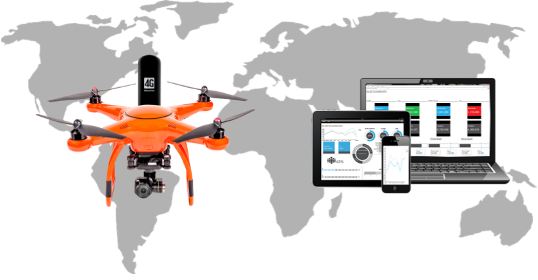
\includegraphics[width=0.95\linewidth]{../img/diy_drone.png}
    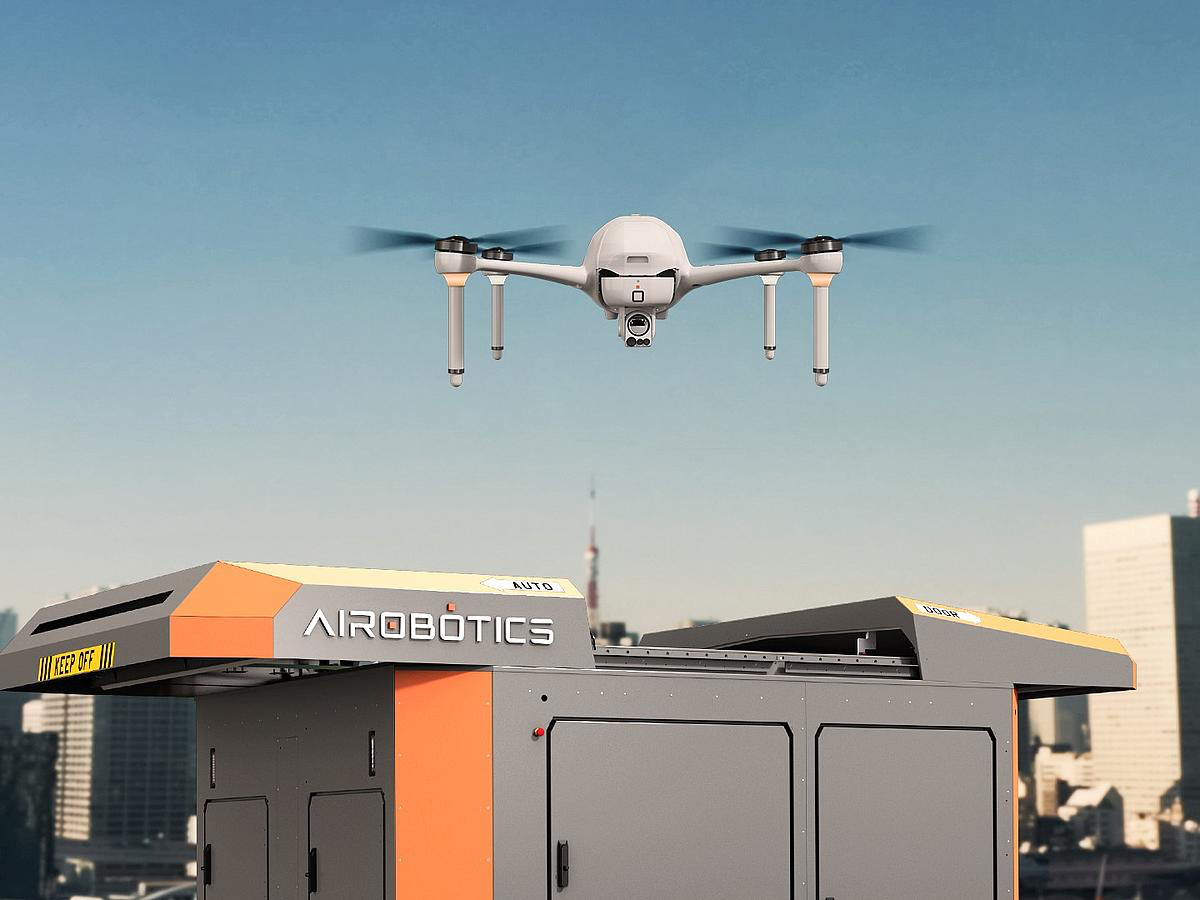
\includegraphics[width=0.95\linewidth]{../img/airbotics.png}
\end{wrapfigure}
\begin{enumerate}
    \item \href{https://habr.com/ru/articles/414121/}{DIY автономный дрон с управлением через интернет} \\
    Обладает широким заявленным функционалом, в том числе описана возможность "посадки в 'точку'".
    Однако, предъявленных результатов данного проекта не обнаружено.

    \item \href{https://www.airoboticsdrones.com}{Airobotics TRUSTED AUTONOMOUS DRONES} \\
    Интеллектуальная сеть дронов, подключенная к центру городского управления.

    \item \href{https://www.dji.com/ru}{ArduPilot} \\
    Open-source проект, предлагающий широкий спектр функций для автоматизации полетов, в том числе точную и безопасную посадку дрона в заданную точку или на площадку.
\end{enumerate}

\paragraph{\underline{Эскиз проекта}:}\
\begin{figure}[h]
    \centering
    \begin{subfigure}{0.4\textwidth}
        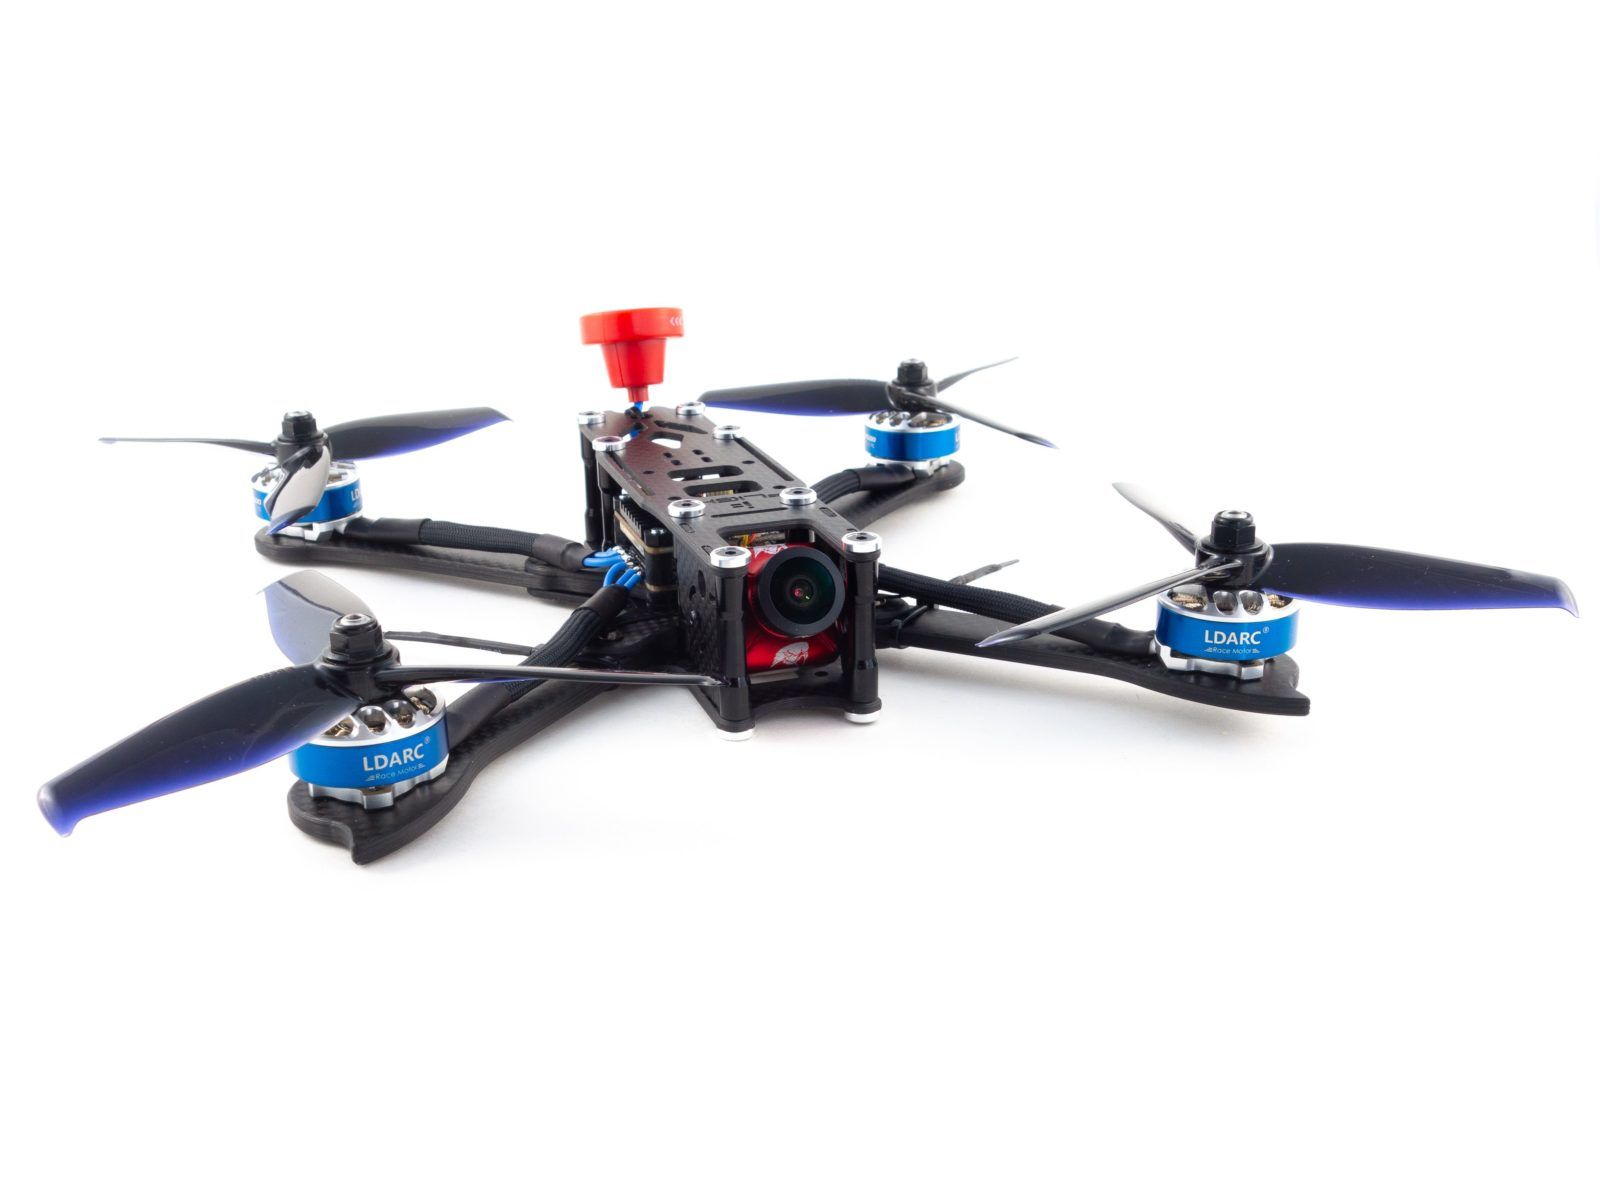
\includegraphics[width=\linewidth]{../img/drone.jpg}
    \end{subfigure}
    \hfill
    \begin{subfigure}{0.2\textwidth}
        
\includegraphics[width=\linewidth]{../img/opencv.png}
    \end{subfigure}
    \hfill
    \begin{subfigure}{0.2\textwidth}
        
\includegraphics[width=\linewidth]{../img/aruco.png}
    \end{subfigure}
\end{figure}

\paragraph{\underline{Элементная база}:}\
\begin{figure}[h]
    \begin{itemize}
        \item Рама 20x20 см - из материалов Физтех Фабрики
        \item Бесколлекторные моторы - DYS 2306 1750KV
        \item Стэк полётный контроллер (контроллер + регуляторы оборотов - плата питания) - Skystars F4
        \item Аккумуляторная батарея - LiPo 3S 3000mAh
        \item Микрокомпьютер - Raspberry Pi 3 Model A+
        \item Модуль камеры для Raspberry Pi 3 - 5MP OV5647
        \item Радиоприемник с пультом управления - Flysky Original FS i6 2,4 ГГц
        \item Соединительные провода и силовой разъем питания XT60
        \item Пропеллеры 5x4.5 - из материалов Физтех Фабрики
    \end{itemize}
\end{figure}

\paragraph{\underline{Медиа}:}\
\begin{figure}[h]
    \centering
    \begin{subfigure}{0.2\textwidth}
    \end{subfigure}
    \hfill
    \centering
    \begin{subfigure}{0.2\textwidth}
        
\includegraphics[width=\linewidth]{../img/tg-qr-code.png}
        \caption*{Telegram}
    \end{subfigure}
    \hfill
    \centering
    \begin{subfigure}{0.2\textwidth}
        
\includegraphics[width=\linewidth]{../img/git-qr-code.png}
        \caption*{GitHub}
    \end{subfigure}
    \hfill
    \centering
    \begin{subfigure}{0.2\textwidth}
    \end{subfigure}
\end{figure}

\end{document}
